\documentclass[a4paper,11pt]{article}
\usepackage[utf8]{inputenc}
\usepackage[T1]{fontenc}
\usepackage{amsmath,amssymb}
\usepackage[a4paper,left=2cm,right=2cm,top=3.6cm,bottom=2.3cm,headheight=1.1cm,headsep=0.6cm,footskip=1cm]{geometry}
\usepackage{xcolor}
\usepackage{tikz}
\usetikzlibrary{calc,arrows.meta,positioning,shapes.geometric,matrix}
\usepackage{fancyhdr}
\usepackage{lastpage}
\usepackage{tabularx}
\usepackage{array}
\usepackage[most]{tcolorbox}
\usepackage{enumitem}
\usepackage{needspace}

% ---------- palet sky (Sky-800 dan Sky-200) ----------
\definecolor{mainc}{HTML}{075985}
\definecolor{accc}{HTML}{0284C7}
\definecolor{skyl}{HTML}{BAE6FD}
\definecolor{deepc}{HTML}{082F49}
\definecolor{softbg}{HTML}{F0F9FF}
\definecolor{warmc}{HTML}{D97706}
\definecolor{brick}{HTML}{B91C1C}
\newcommand{\dis}{\displaystyle}
\newcommand{\dd}[2]{\dfrac{d#1}{d#2}}
\newcolumntype{C}[1]{>{\centering\arraybackslash}p{#1}}

\setlength{\parindent}{0pt}
\renewcommand{\arraystretch}{1.35}

\tikzset{
  ar/.style={-{Stealth[length=1.8mm]},thick,mainc},
  box/.style={draw=mainc,thick,rounded corners=3pt,fill=softbg,align=center,inner sep=4pt},
  ax/.style={-{Stealth[length=1.8mm]},thick,mainc}
}

% ---------- header ----------
\pagestyle{fancy}
\fancyhf{}
\renewcommand{\headrulewidth}{0pt}
\fancyhead[L]{%
  \begin{tikzpicture}[remember picture,overlay]
    \fill[mainc] ([yshift=-1.2cm]current page.north west) rectangle ([yshift=-3.15cm]current page.north east);
    \fill[skyl] ([yshift=-3.15cm]current page.north west) rectangle ([yshift=-3.3cm]current page.north east);
  \end{tikzpicture}%
  \color{white}\bfseries\large Latihan Soal Turunan}
\fancyhead[R]{\color{white}\small Diunduh dari website \textbf{Math1729}\ \,|\,\ 5 Oktober 2026}
\fancyfoot[L]{\small\color{mainc}Math1729 --- Turunan}
\fancyfoot[R]{\small\color{mainc}Halaman \thepage\ dari \pageref{LastPage}}

% ---------- komponen ----------
\newcounter{no}
\newcommand{\bagian}[2]{\par\Needspace{6\baselineskip}\vspace{1.0em}\noindent
  \begin{tcolorbox}[colback=mainc,colframe=mainc,coltext=white,boxrule=0pt,arc=2pt,left=6pt,right=6pt,top=3pt,bottom=3pt]
  \textbf{#1}\hfill{\small #2}\end{tcolorbox}\setcounter{no}{0}\par\vspace{-0.3em}}
\newcommand{\tingkat}[2]{\par\Needspace{7\baselineskip}\vspace{0.6em}\noindent
  {\color{accc}\rule{3pt}{1.1em}}\ {\color{mainc}\bfseries #1}\ {\small\color{gray}--- #2}\par\vspace{0.1em}}
\newcommand{\soal}[2]{\par\vspace{0.75em}\stepcounter{no}\noindent
  \begin{minipage}[t]{1.8em}\textbf{\theno.}\end{minipage}%
  \begin{minipage}[t]{\dimexpr\linewidth-1.8em\relax}#1\par\vspace{0.35em}#2\end{minipage}\par}
\newcommand{\poin}[1]{\hfill{\small\color{mainc}[#1 poin]}}
\newcommand{\gbr}[2]{\noindent\begin{minipage}[t]{0.56\linewidth}#1\end{minipage}\hfill\raisebox{\ht\strutbox}{\begin{minipage}[t]{0.41\linewidth}\vspace{0pt}\centering#2\end{minipage}}}
\newcommand{\pil}[5]{\begin{tabularx}{\linewidth}{@{}*{5}{X}@{}}\textbf{A.}\;#1 & \textbf{B.}\;#2 & \textbf{C.}\;#3 & \textbf{D.}\;#4 & \textbf{E.}\;#5\end{tabularx}}
\newcommand{\pilx}[5]{\begin{tabularx}{\linewidth}{@{}*{3}{X}@{}}\textbf{A.}\;#1 & \textbf{B.}\;#2 & \textbf{C.}\;#3\\[10pt] \textbf{D.}\;#4 & \textbf{E.}\;#5 & \end{tabularx}}
\newcommand{\pilv}[5]{\begin{tabularx}{\linewidth}{@{}lX@{}}\textbf{A.} & #1\\ \textbf{B.} & #2\\ \textbf{C.} & #3\\ \textbf{D.} & #4\\ \textbf{E.} & #5\end{tabularx}}
\newcommand{\mk}[1]{\begin{tabularx}{\linewidth}{|C{0.9cm}|X|C{1.4cm}|C{1.4cm}|}\hline \textbf{No}&\textbf{Pernyataan}&\textbf{Benar}&\textbf{Salah}\\ \hline #1\end{tabularx}}
\newcommand{\mkr}[2]{#1&#2&$\bigcirc$&$\bigcirc$\\ \hline}
\newcommand{\jwb}{\hfill Jawaban: \rule{4.5cm}{0.4pt}}
\begin{document}
\thispagestyle{fancy}

\begin{center}
  {\color{mainc}\fontsize{22}{26}\selectfont\bfseries Latihan Soal Turunan\par}
  \vspace{2pt}
  {\color{accc}\large Aturan Turunan, Garis Singgung, Fungsi Naik--Turun, Nilai Ekstrem, Kecekungan, dan Penalaran Optimasi\par}
\end{center}
\vspace{2pt}
\begin{tcolorbox}[colback=softbg,colframe=mainc!40,boxrule=0.6pt,arc=3pt,left=8pt,right=8pt,top=5pt,bottom=5pt]
\noindent\textbf{Nama} : \rule{4.6cm}{0.4pt}\hfill\textbf{Kelas} : \rule{2.2cm}{0.4pt}\hfill\textbf{Skor} : \rule{2.2cm}{0.4pt}
\end{tcolorbox}
\vspace{2pt}
\begin{tcolorbox}[colback=white,colframe=accc,boxrule=0.8pt,arc=3pt,left=8pt,right=8pt,top=4pt,bottom=4pt,title={\bfseries Petunjuk Pengerjaan},coltitle=white,fonttitle=\small]
\small
\begin{enumerate}[leftmargin=1.4em,itemsep=1pt,topsep=1pt]
\item Soal terdiri atas \textbf{20 pilihan ganda} (5 mudah, 6 sedang, 7 sulit, 2 HOTS), \textbf{5 isian singkat} (2 sedang, 3 sulit), dan \textbf{5 uraian (essay)} (2 sedang, 2 sulit, 1 HOTS). Soal disusun berjenjang dan memakai bentuk yang sejalan dengan UTBK-SNBT 2026: pilihan ganda lima opsi, pilihan majemuk kompleks (tabel pernyataan benar/salah), kecukupan data, soal berkonteks dengan gambar atau grafik, serta isian singkat. Soal HOTS menuntut proses \emph{merumuskan}, \emph{menggunakan}, dan \emph{menafsirkan} model matematika. Alokasi waktu yang disarankan: 120 menit.
\item Skor: pilihan ganda 2 poin, isian singkat 4 poin, uraian 8 poin per soal (total 100 poin). Pada soal pilihan majemuk kompleks (berbentuk tabel), skor diberikan jika \textbf{semua baris} dijawab benar. Tidak ada pengurangan skor untuk jawaban salah.
\item Notasi: $f'(x)$, $y'$, dan $\dd yx$ menyatakan turunan pertama; $f^{(n)}$ menyatakan turunan ke-$n$. Sudut diukur dalam radian. Gunakan $e\approx2{,}72$, $\ln2\approx0{,}69$, dan $\pi\approx3{,}14$ bila diperlukan. Gambar tidak selalu digambar sesuai skala.
\item Bilangan ribuan ditulis dengan tanda titik dan bilangan desimal dengan tanda koma. Pada isian singkat, tuliskan hanya jawaban akhir (boleh dalam bentuk akar, pecahan, atau $\ln$).
\item Kalkulator tidak diperkenankan.
\end{enumerate}
\end{tcolorbox}

% =====================================================================
\bagian{A. Pilihan Ganda}{20 soal $\times$ 2 poin = 40 poin. Pilih satu jawaban yang paling tepat.}

\tingkat{Tingkat Mudah}{soal 1 sampai 5}
\soal{\gbr{Gambar menunjukkan grafik fungsi $y=f(x)$ dan garis $g$ yang menyinggung grafik di titik $A(2,5)$. Garis $g$ memotong sumbu $y$ di titik $(0,1)$. Nilai $f(2)+f'(2)$ adalah \dots.}{%
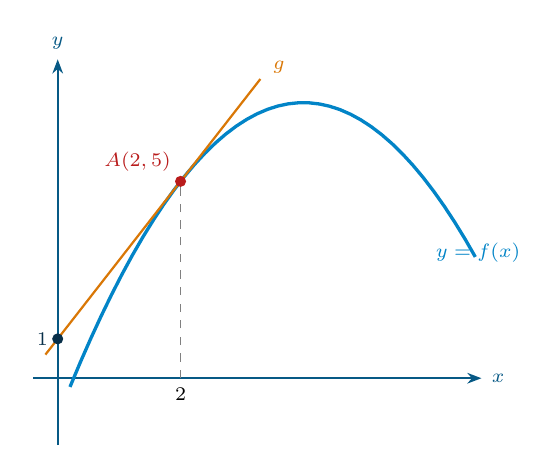
\begin{tikzpicture}[x=0.78cm,y=0.5cm]
\draw[ax] (-0.4,0)--(6.9,0) node[right,font=\scriptsize]{$x$};
\draw[ax] (0,-1.7)--(0,8.1) node[above,font=\scriptsize]{$y$};
\draw[accc,very thick,domain=0.2:6.8,samples=40] plot(\x,{-0.5*\x*\x+4*\x-1});
\draw[warmc,thick,domain=-0.2:3.3] plot(\x,{2*\x+1});
\draw[gray,dashed] (2,0)--(2,5);
\fill[brick] (2,5) circle (2pt) node[above left,font=\scriptsize]{$A(2,5)$};
\fill[deepc] (0,1) circle (2pt) node[left,font=\scriptsize]{$1$};
\node[font=\scriptsize,below] at (2,0) {$2$};
\node[font=\scriptsize,accc,right] at (6.0,3.2) {$y=f(x)$};
\node[font=\scriptsize,warmc] at (3.6,7.9) {$g$};
\end{tikzpicture}}}{\pil{$3$}{$5$}{$\frac{11}2$}{$6$}{$7$}}
\soal{Diketahui $f(x)=\dfrac{x^3-8}{x-2}$ untuk $x\neq2$. Nilai $f'(1)$ adalah \dots.}{\pil{$2$}{$3$}{$4$}{$6$}{$8$}}
\soal{Jika $f(x)=2\sin x-\cos 3x$, maka $f'\!\left(\dfrac\pi2\right)$ adalah \dots.}{\pil{$-3$}{$-1$}{$0$}{$1$}{$3$}}
\soal{Posisi sebuah benda yang bergerak pada garis lurus dinyatakan oleh $s(t)=t^3-6t^2+9t$ dengan $s$ dalam meter dan $t$ dalam detik. Pada saat $t=2$ detik, benda tersebut \dots.}{\pilv{bergerak dengan kecepatan $3$ m/s ke arah positif}{bergerak dengan kecepatan $3$ m/s ke arah negatif}{berhenti sesaat}{bergerak dengan kecepatan $12$ m/s ke arah negatif}{bergerak dengan kecepatan $2$ m/s ke arah positif}}
\soal{Diketahui $f(x)=x\,|x|$. Tentukan nilai kebenaran setiap pernyataan berikut dengan menandai kolom Benar atau Salah.}{\mk{%
\mkr{1}{$f$ kontinu di $x=0$.}
\mkr{2}{Turunan kiri dan turunan kanan $f$ di $x=0$ tidak sama.}
\mkr{3}{$f'(-2)=-4$.}
\mkr{4}{$f'(x)=2|x|$ untuk setiap bilangan real $x$.}}}

\tingkat{Tingkat Sedang}{soal 6 sampai 11}
\soal{Jika $f(x)=\sqrt{1+\sin^2x}$, maka $f'\!\left(\dfrac\pi4\right)$ adalah \dots.}{\pil{$\frac{\sqrt6}{12}$}{$\frac14$}{$\frac{\sqrt2}{4}$}{$\frac{\sqrt6}{6}$}{$\frac{\sqrt6}{3}$}}
\soal{\gbr{Gambar menunjukkan grafik $y=f'(x)$, yaitu turunan pertama fungsi $f$. Grafik tersebut memotong sumbu $x$ di $x=1$ dan $x=3$, serta menyinggung sumbu $x$ di $x=-2$. Pernyataan yang benar tentang fungsi $f$ adalah \dots.}{%
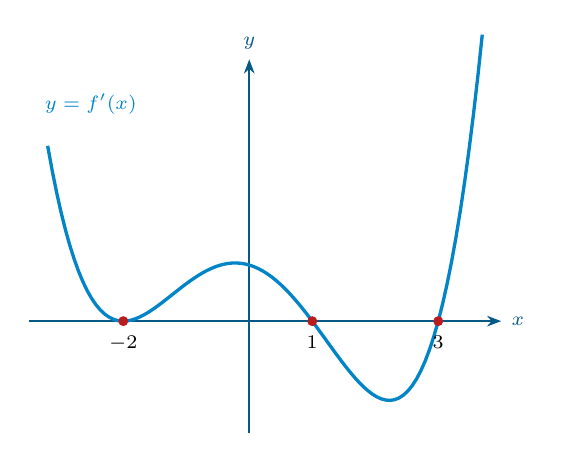
\begin{tikzpicture}[x=0.8cm,y=0.95cm]
\draw[ax] (-3.5,0)--(4.0,0) node[right,font=\scriptsize]{$x$};
\draw[ax] (0,-1.5)--(0,3.5) node[above,font=\scriptsize]{$y$};
\draw[accc,very thick,domain=-3.2:3.7,samples=100] plot(\x,{(\x+2)^2*(\x-1)*(\x-3)/16});
\foreach \p in {-2,1,3}{\fill[brick] (\p,0) circle (1.8pt); \node[font=\scriptsize,below=2pt] at (\p,0) {$\p$};}
\node[font=\scriptsize,accc,right] at (-3.4,2.9) {$y=f'(x)$};
\end{tikzpicture}}}{\pilv{$f$ mempunyai maksimum lokal di $x=-2$ dan minimum lokal di $x=3$.}{$f$ mempunyai maksimum lokal di $x=1$ dan minimum lokal di $x=3$, sedangkan $x=-2$ bukan titik ekstrem.}{$f$ mempunyai tiga titik ekstrem lokal, yaitu di $x=-2$, $x=1$, dan $x=3$.}{$f$ turun pada $x<1$ dan naik pada $1<x<3$.}{$f$ mempunyai minimum lokal di $x=1$ dan maksimum lokal di $x=3$.}}
\soal{Kurva $y^3+xy=2x^2$ melalui titik $(1,1)$. Persamaan garis normal kurva di titik tersebut adalah \dots.}{\pilx{$4x+3y=7$}{$3x-4y=-1$}{$3x+4y=7$}{$4x-3y=1$}{$x+y=2$}}
\soal{\gbr{Tabel di samping memuat nilai fungsi $f$, $g$, dan turunannya di beberapa titik. Jika $P(x)=x^2\,f\big(g(x)\big)$, maka $P'(2)$ adalah \dots.}{%
\small\renewcommand{\arraystretch}{1.25}
\begin{tabular}{|c|c|c|c|c|}\hline
$x$ & $f(x)$ & $f'(x)$ & $g(x)$ & $g'(x)$\\ \hline
$1$ & $2$ & $4$ & $3$ & $-1$\\ \hline
$2$ & $3$ & $-2$ & $1$ & $6$\\ \hline
$3$ & $1$ & $5$ & $2$ & $2$\\ \hline
\end{tabular}}}{\pil{$-40$}{$24$}{$96$}{$104$}{$108$}}
\soal{Fungsi $f(x)=x^3+ax^2+3ax+5$ monoton naik pada seluruh bilangan real (yaitu $f(x_1)<f(x_2)$ jika $x_1<x_2$). Banyak bilangan bulat $a$ yang memenuhi adalah \dots.}{\pil{$8$}{$9$}{$10$}{$18$}{$19$}}
\soal{Untuk $f(x)=\ln\!\left(e^{2x}+e^{-2x}\right)$, nilai $f'(\ln\sqrt3)$ adalah \dots.}{\pil{$\frac45$}{$1$}{$\frac65$}{$\frac32$}{$\frac85$}}

\tingkat{Tingkat Sulit}{soal 12 sampai 18, setara UTBK}
\soal{Grafik fungsi $f(x)=ax^3+bx^2+cx+d$ memotong sumbu $y$ di titik $(0,5)$ dan mempunyai titik belok $(1,3)$. Gradien garis singgung grafik di titik belok tersebut adalah $-3$. Selisih nilai maksimum lokal dan nilai minimum lokal $f$ adalah \dots.}{\pil{$1$}{$3$}{$4$}{$5$}{$6$}}
\soal{\gbr{Gambar memperlihatkan parabola $y=x^2$ dan $y=-(x-2)^2$ beserta dua garis singgung persekutuannya, yaitu $\ell_1$ dan $\ell_2$. Luas daerah segitiga yang dibatasi oleh $\ell_1$, $\ell_2$, dan sumbu $y$ adalah \dots\ satuan luas.}{%
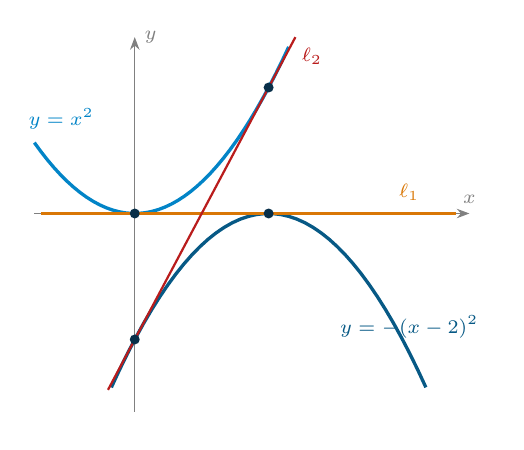
\begin{tikzpicture}[x=0.85cm,y=0.4cm]
\clip (-1.6,-6.6) rectangle (5.4,5.9);
\draw[gray,-{Stealth[length=1.6mm]}] (0,-6.3)--(0,5.6) node[right,font=\scriptsize]{$y$};
\draw[gray,-{Stealth[length=1.6mm]}] (-1.5,0)--(5.0,0) node[above,font=\scriptsize]{$x$};
\draw[accc,very thick,domain=-1.5:2.3,samples=40] plot(\x,{\x*\x});
\draw[mainc,very thick,domain=-0.35:4.35,samples=40] plot(\x,{-(\x-2)*(\x-2)});
\draw[warmc,thick] (-1.4,0)--(4.8,0);
\draw[brick,thick,domain=-0.4:2.4] plot(\x,{4*\x-4});
\fill[deepc] (0,0) circle (1.8pt) (2,0) circle (1.8pt) (2,4) circle (1.8pt) (0,-4) circle (1.8pt);
\node[font=\scriptsize,warmc,above] at (4.1,0.1) {$\ell_1$};
\node[font=\scriptsize,brick,right] at (2.35,5.0) {$\ell_2$};
\node[font=\scriptsize,accc] at (-1.1,3.0) {$y=x^2$};
\node[font=\scriptsize,mainc] at (4.1,-3.6) {$y=-(x-2)^2$};
\end{tikzpicture}}}{\pil{$1$}{$2$}{$4$}{$8$}{$16$}}
\soal{\gbr{Lampu jalan dipasang pada puncak tiang setinggi $6$ m. Dina, yang tingginya $1{,}5$ m, berjalan menjauhi tiang dengan kecepatan tetap $1{,}2$ m/s (lihat gambar). Pada saat Dina berada $9$ m dari tiang, panjang bayangannya bertambah dengan laju \dots\ m/s.}{%
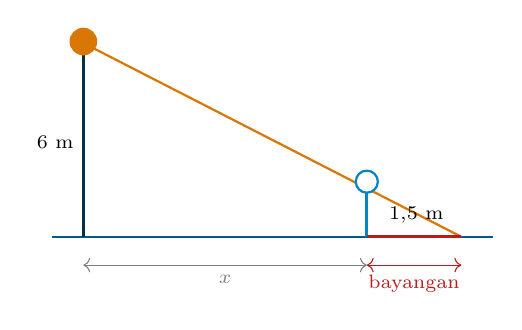
\begin{tikzpicture}[x=0.4cm,y=0.4cm]
\draw[mainc,thick] (-1,0)--(13,0);
\draw[deepc,very thick] (0,0)--(0,6);
\fill[warmc] (0,6.2) circle (5pt);
\draw[warmc,thick] (0.1,6.1)--(12,0);
\draw[accc,very thick] (9,0)--(9,1.4);
\draw[accc,thick,fill=white] (9,1.75) circle (0.35);
\draw[brick,very thick] (9,0)--(12,0);
\draw[<->,gray] (0,-0.9)--(9,-0.9) node[midway,below,font=\scriptsize]{$x$};
\draw[<->,brick] (9,-0.9)--(12,-0.9) node[midway,below,font=\scriptsize,brick]{bayangan};
\node[font=\scriptsize,left] at (0,3) {$6$ m};
\node[font=\scriptsize,right] at (9.4,0.7) {$1{,}5$ m};
\end{tikzpicture}}}{\pil{$0{,}3$}{$0{,}4$}{$1{,}2$}{$1{,}6$}{$2{,}0$}}
\soal{\gbr{Selembar seng selebar $30$ cm dilipat menjadi talang air. Penampang talang berbentuk trapesium sama kaki dengan alas $10$ cm dan kedua sisi miring masing-masing $10$ cm. Setiap sisi miring membentuk sudut $\theta$ terhadap perpanjangan alas, dengan $0<\theta<\frac\pi2$ (lihat gambar). Luas penampang maksimum talang tersebut adalah \dots\ cm$^2$.}{%
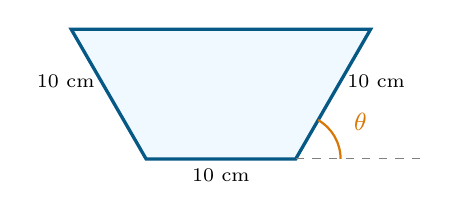
\begin{tikzpicture}[scale=1.9]
\coordinate (A) at (-0.5,0); \coordinate (B) at (0.5,0);
\coordinate (C) at ({0.5+cos(60)},{sin(60)}); \coordinate (D) at ({-0.5-cos(60)},{sin(60)});
\draw[mainc,very thick,fill=softbg] (A)--(B)--(C)--(D)--cycle;
\draw[gray,dashed] (B)--(1.35,0);
\draw[warmc,thick] (0.8,0) arc (0:60:0.3);
\node[font=\small,warmc] at ({0.5+0.5*cos(30)},{0.5*sin(30)}) {$\theta$};
\node[font=\scriptsize,below] at (0,0) {$10$ cm};
\node[font=\scriptsize,right] at (0.78,0.52) {$10$ cm};
\node[font=\scriptsize,left] at (-0.78,0.52) {$10$ cm};
\end{tikzpicture}}}{\pil{$75\sqrt3$}{$100$}{$50\sqrt3$}{$75$}{$100\sqrt3$}}
\soal{Fungsi $f(x)=(ax+b)e^{-x}$ mempunyai grafik yang melalui titik $(0,-2)$ dan mempunyai titik stasioner di $x=3$. Ordinat titik belok grafik $f$ adalah \dots.}{\pil{$\dfrac1{e^4}$}{$\dfrac1{e^3}$}{$\dfrac3{e^4}$}{$\dfrac2{e^3}$}{$\dfrac2{e^4}$}}
\soal{\gbr{Gambar menunjukkan grafik fungsi $f$ yang dapat diturunkan dua kali. Titik $P$ dan $R$ adalah titik ekstrem lokal, sedangkan titik $Q$ adalah titik belok. Tentukan nilai kebenaran setiap pernyataan berikut dengan menandai kolom Benar atau Salah.}{%
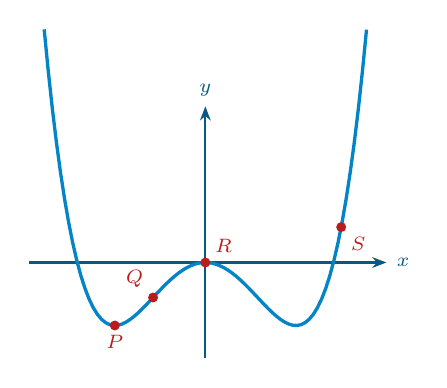
\begin{tikzpicture}[x=1.15cm,y=3.2cm]
\draw[ax] (-1.95,0)--(2.0,0) node[right,font=\scriptsize]{$x$};
\draw[ax] (0,-0.38)--(0,0.62) node[above,font=\scriptsize]{$y$};
\draw[accc,very thick,domain=-1.78:1.78,samples=80] plot(\x,{\x*\x*\x*\x/4-\x*\x/2});
\fill[brick] (-1,-0.25) circle (1.8pt) node[below,font=\scriptsize]{$P$};
\fill[brick] (-0.57735,-0.13889) circle (1.8pt) node[above left,font=\scriptsize]{$Q$};
\fill[brick] (0,0) circle (1.8pt) node[above right,font=\scriptsize]{$R$};
\fill[brick] (1.5,0.1406) circle (1.8pt) node[below right,font=\scriptsize]{$S$};
\end{tikzpicture}}}{\mk{%
\mkr{1}{Di titik $P$: $f'(x)=0$ dan $f''(x)>0$.}
\mkr{2}{Di titik $Q$: $f'(x)<0$ dan $f''(x)=0$.}
\mkr{3}{Di titik $R$: $f'(x)=0$ dan $f''(x)<0$.}
\mkr{4}{Di titik $S$: $f'(x)>0$ dan $f''(x)<0$.}}}
\soal{Jika $f(x)=\sin^2x$, maka $f^{(2025)}\!\left(\dfrac\pi4\right)$ adalah \dots.}{\pil{$0$}{$2^{2023}$}{$2^{2024}$}{$2^{2025}$}{$-2^{2024}$}}

\Needspace{16\baselineskip}
\tingkat{Tingkat HOTS}{soal 19 dan 20, penalaran tingkat tinggi gaya UTBK}
\soal{Diketahui $f(x)=ax^3+bx^2+cx+d$ dengan $a,b,c,d$ bilangan real. Apakah grafik $f$ mempunyai \textbf{tepat satu} titik belok?
\begin{enumerate}[label=(\arabic*),leftmargin=1.8em,itemsep=0pt,topsep=2pt]
\item Persamaan $f'(x)=0$ mempunyai tepat dua akar real yang berbeda.
\item Persamaan $f(x)=0$ mempunyai tepat tiga akar real yang berbeda.
\end{enumerate}}{\begin{tabularx}{\linewidth}{@{}lX@{}}
\textbf{A.} & Pernyataan (1) SAJA cukup untuk menjawab pertanyaan, tetapi pernyataan (2) SAJA tidak cukup.\\
\textbf{B.} & Pernyataan (2) SAJA cukup untuk menjawab pertanyaan, tetapi pernyataan (1) SAJA tidak cukup.\\
\textbf{C.} & DUA pernyataan BERSAMA-SAMA cukup untuk menjawab pertanyaan, tetapi SATU pernyataan SAJA tidak cukup.\\
\textbf{D.} & Pernyataan (1) SAJA cukup dan pernyataan (2) SAJA cukup untuk menjawab pertanyaan.\\
\textbf{E.} & Pernyataan (1) dan pernyataan (2) tidak cukup untuk menjawab pertanyaan.
\end{tabularx}}
\soal{\gbr{Pembangkit listrik berada di titik $A$ pada garis pantai yang lurus. Sebuah pulau $B$ berjarak $6$ km dari pantai, tepat di depan titik $D$ dengan $AD=8$ km. Kabel akan dipasang dari $A$ menyusuri daratan sampai titik $P$ di antara $A$ dan $D$, kemudian menembus laut langsung ke $B$. Biaya pemasangan kabel di darat Rp3 juta per km dan di laut Rp5 juta per km. Biaya minimum pemasangan seluruh kabel adalah \dots\ juta rupiah.}{%
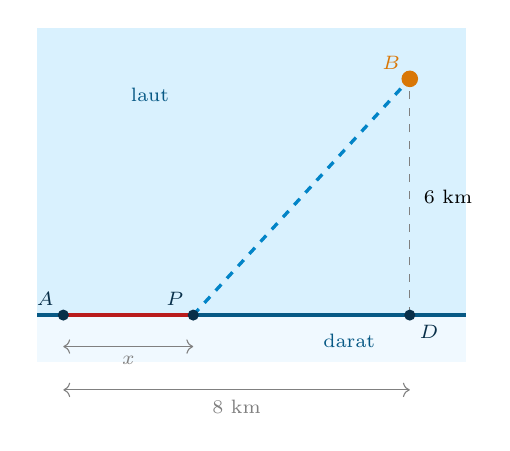
\begin{tikzpicture}[x=0.55cm,y=0.5cm]
\fill[skyl!55] (-0.6,0) rectangle (9.3,7.3);
\fill[softbg] (-0.6,-1.2) rectangle (9.3,0);
\draw[mainc,very thick] (-0.6,0)--(9.3,0);
\draw[brick,very thick] (0,0)--(3,0);
\draw[accc,very thick,dashed] (3,0)--(8,6);
\draw[gray,dashed] (8,0)--(8,6);
\fill[deepc] (0,0) circle (2pt) node[above left,font=\scriptsize]{$A$};
\fill[deepc] (3,0) circle (2pt) node[above left,font=\scriptsize]{$P$};
\fill[deepc] (8,0) circle (2pt) node[below right,font=\scriptsize]{$D$};
\fill[warmc] (8,6) circle (3pt) node[above left,font=\scriptsize]{$B$};
\draw[<->,gray] (0,-0.8)--(3,-0.8) node[midway,below,font=\scriptsize]{$x$};
\draw[<->,gray] (0,-1.9)--(8,-1.9) node[midway,below,font=\scriptsize]{$8$ km};
\node[font=\scriptsize,right] at (8.1,3) {$6$ km};
\node[font=\scriptsize,mainc] at (2.0,5.6) {laut};
\node[font=\scriptsize,mainc] at (6.6,-0.65) {darat};
\end{tikzpicture}}}{\pil{$46$}{$50$}{$52$}{$48$}{$54$}}

% =====================================================================
\bagian{B. Isian Singkat}{5 soal $\times$ 4 poin = 20 poin. Tuliskan hanya jawaban akhir.}

\tingkat{Tingkat Sedang}{soal 1 dan 2}
\soal{Posisi sebuah partikel pada garis lurus dinyatakan oleh $s(t)=2t^3-21t^2+60t$ dengan $s$ dalam meter dan $t\ge0$ dalam detik. Percepatan partikel (dalam m/s$^2$) pada saat partikel berhenti sesaat untuk \textbf{kedua kalinya} adalah \dots.}{\jwb}
\soal{Garis $y=9x+k$ menyinggung kurva $y=x^3-3x^2$ untuk dua nilai $k$ yang berbeda. Selisih kedua nilai $k$ tersebut (nilai terbesar dikurangi nilai terkecil) adalah \dots.}{\jwb}

\tingkat{Tingkat Sulit}{soal 3 sampai 5}
\soal{Nilai minimum fungsi $f(x)=\sqrt{x^2+4}+\sqrt{x^2-12x+45}$ untuk $x\in\mathbb R$ adalah \dots.}{\jwb}
\soal{\gbr{Titik $P(1,2)$ terletak pada kurva $x^2-xy+y^2=3$ (lihat gambar). Nilai $\dfrac{d^2y}{dx^2}$ di titik $P$ adalah \dots.}{%
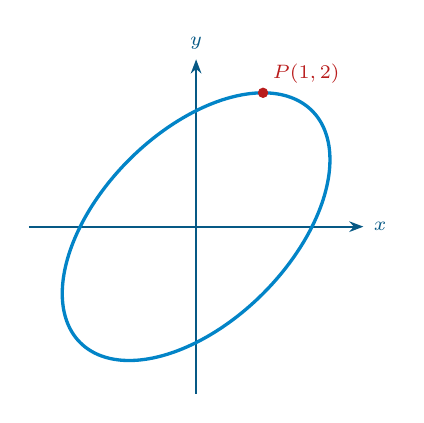
\begin{tikzpicture}[scale=0.85]
\draw[ax] (-2.5,0)--(2.5,0) node[right,font=\scriptsize]{$x$};
\draw[ax] (0,-2.5)--(0,2.5) node[above,font=\scriptsize]{$y$};
\draw[accc,very thick,smooth,samples=120,domain=0:360] plot ({sqrt(3)*cos(\x)-sin(\x)},{sqrt(3)*cos(\x)+sin(\x)});
\fill[brick] (1,2) circle (2.2pt) node[above right,font=\scriptsize]{$P(1,2)$};
\end{tikzpicture}}}{\jwb}
\soal{Jika $f(x)=(x^2+1)^x$, maka nilai $f'(1)$ adalah \dots.}{\jwb}

% =====================================================================
\Needspace{16\baselineskip}
\bagian{C. Uraian (Essay)}{5 soal $\times$ 8 poin = 40 poin. Tuliskan langkah penyelesaian dengan lengkap.}

\tingkat{Tingkat Sedang}{soal 1 dan 2}
\soal{\gbr{Sebuah jendela berbentuk persegi panjang dengan setengah lingkaran di bagian atasnya (lihat gambar). Lebar persegi panjang adalah $2r$ meter dan tingginya $h$ meter. Kerangka luar jendela (alas, dua sisi tegak, dan busur setengah lingkaran) dibuat dari bahan sepanjang $10$ m.\par\smallskip
(a) Nyatakan $h$ dalam $r$, lalu tuliskan luas jendela $A(r)$ beserta batas nilai $r$.\par
(b) Tentukan $r$ yang membuat $A$ maksimum, lalu buktikan bahwa nilai itu memang maksimum dengan uji turunan kedua.\par
(c) Tentukan luas maksimum (dalam $\pi$) dan tunjukkan bahwa pada saat itu $h=r$.\par
(d) Hitung $A$ pada kedua ujung batas nilai $r$ dan simpulkan apakah maksimum pada (b) merupakan maksimum mutlak.}{%
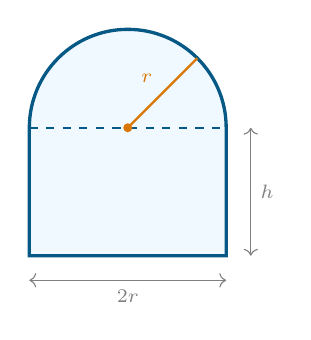
\begin{tikzpicture}[scale=1.25]
\draw[mainc,very thick,fill=softbg] (-1,0)--(1,0)--(1,1.3) arc (0:180:1)--(-1,0)--cycle;
\draw[mainc,thick,dashed] (-1,1.3)--(1,1.3);
\draw[<->,gray] (-1,-0.25)--(1,-0.25) node[midway,below,font=\scriptsize]{$2r$};
\draw[<->,gray] (1.25,0)--(1.25,1.3) node[midway,right,font=\scriptsize]{$h$};
\draw[warmc,thick] (0,1.3)--(0.707,2.007) node[midway,above left,font=\scriptsize]{$r$};
\fill[warmc] (0,1.3) circle (1.3pt);
\end{tikzpicture}}}{\poin{8}}
\soal{\gbr{Secangkir teh bersuhu $100^\circ$C diletakkan di ruangan yang bersuhu $25^\circ$C. Suhu teh setelah $t$ menit dinyatakan oleh $T(t)=25+75e^{-t/10}$ (dalam $^\circ$C). Gambar memperlihatkan grafik $T$ dan garis singgungnya di $t=0$.\par\smallskip
(a) Tentukan $T'(t)$ dan tafsirkan makna $T'(0)$ beserta satuannya.\par
(b) Pada menit ke berapa laju penurunan suhu tepat $3{,}75^\circ$C per menit? Berapa suhu teh saat itu?\par
(c) Tentukan $T''(t)$, tunjukkan $T''(t)>0$, lalu jelaskan artinya terhadap laju pendinginan.\par
(d) Tunjukkan bahwa garis singgung di $t=0$ memotong garis $T=25$ di $t=10$. Dengan hasil (c), jelaskan mengapa pada $t=10$ suhu teh sebenarnya masih di atas $25^\circ$C.}{%
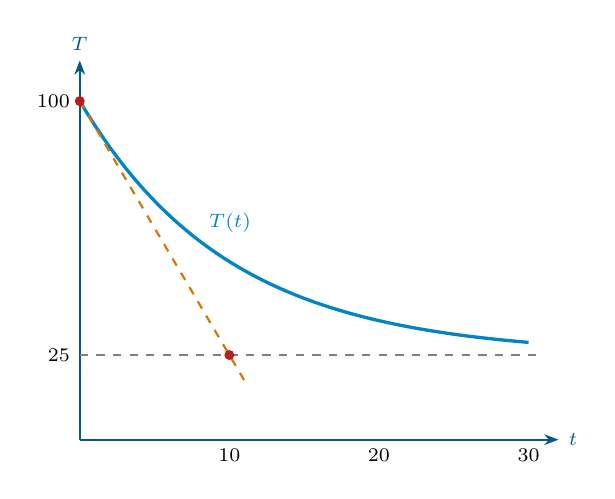
\begin{tikzpicture}[x=0.19cm,y=0.043cm]
\draw[ax] (0,0)--(32,0) node[right,font=\scriptsize]{$t$};
\draw[ax] (0,0)--(0,112) node[above,font=\scriptsize]{$T$};
\draw[gray,dashed] (0,25)--(31,25);
\draw[accc,very thick,domain=0:30,samples=60] plot(\x,{25+75*exp(-\x/10)});
\draw[warmc,thick,dashed] (0,100)--(11,17.5);
\fill[brick] (0,100) circle (1.8pt); \fill[brick] (10,25) circle (1.8pt);
\node[font=\scriptsize,left] at (0,100) {$100$};
\node[font=\scriptsize,left] at (0,25) {$25$};
\node[font=\scriptsize,below] at (10,0) {$10$};
\node[font=\scriptsize,below] at (20,0) {$20$};
\node[font=\scriptsize,below] at (30,0) {$30$};
\node[font=\scriptsize,accc,right] at (8,64) {$T(t)$};
\end{tikzpicture}}}{\poin{8}}

\Needspace{22\baselineskip}
\tingkat{Tingkat Sulit}{soal 3 dan 4}
\soal{\gbr{Pada gambar, titik $P(t,\tfrac1t)$ dengan $t>0$ terletak pada kurva $y=\dfrac1x$. Garis singgung kurva di $P$ memotong sumbu $x$ di $A$ dan sumbu $y$ di $B$.\par\smallskip
(a) Tunjukkan bahwa persamaan garis singgung di $P$ adalah $y=-\dfrac{x}{t^2}+\dfrac2t$.\par
(b) Tentukan koordinat $A$ dan $B$, lalu tunjukkan bahwa $P$ adalah titik tengah ruas $AB$.\par
(c) Tunjukkan bahwa luas segitiga $OAB$ bernilai tetap untuk setiap $t>0$.\par
(d) Tentukan nilai $t$ yang membuat panjang $AB$ minimum, kemudian hitung panjang minimum tersebut.}{%
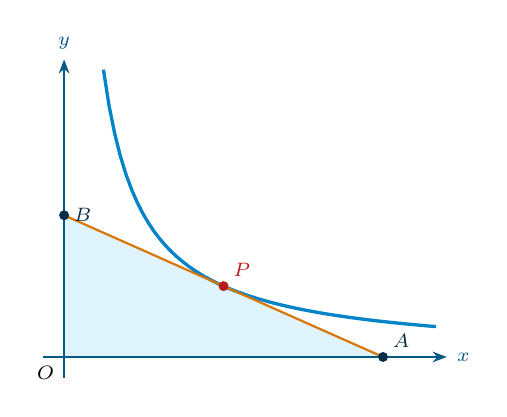
\begin{tikzpicture}[x=1.35cm,y=1.35cm]
\fill[skyl!45] (0,0)--(3,0)--(0,1.3333)--cycle;
\draw[ax] (-0.2,0)--(3.6,0) node[right,font=\scriptsize]{$x$};
\draw[ax] (0,-0.2)--(0,2.8) node[above,font=\scriptsize]{$y$};
\draw[accc,very thick,domain=0.37:3.5,samples=60] plot(\x,{1/\x});
\draw[warmc,thick] (0,1.3333)--(3,0);
\fill[brick] (1.5,0.6667) circle (1.8pt) node[above right,font=\scriptsize]{$P$};
\fill[deepc] (3,0) circle (1.8pt) node[above right,font=\scriptsize]{$A$};
\fill[deepc] (0,1.3333) circle (1.8pt) node[right,font=\scriptsize]{$B$};
\node[font=\scriptsize,below left] at (0,0) {$O$};
\end{tikzpicture}}}{\poin{8}}
\soal{\gbr{Sebuah tangki berbentuk kerucut terbalik (puncak di bawah) dengan jari-jari atas $3$ m dan tinggi $6$ m, mula-mula kosong. Air dialirkan masuk dengan laju tetap $2$ m$^3$/menit dan sekaligus bocor melalui lubang di dasar dengan laju $\frac h2$ m$^3$/menit, dengan $h$ adalah tinggi air (dalam meter) saat itu.\par\smallskip
(a) Tunjukkan bahwa volume air adalah $V=\dfrac{\pi}{12}h^3$.\par
(b) Tunjukkan bahwa $\dd ht=\dfrac{8-2h}{\pi h^2}$, lalu hitung nilainya saat $h=2$.\par
(c) Tentukan laju perubahan luas permukaan air saat $h=2$.\par
(d) Tentukan tinggi $h$ saat $\dd ht=0$. Apakah tangki akan meluap? Jelaskan.}{%
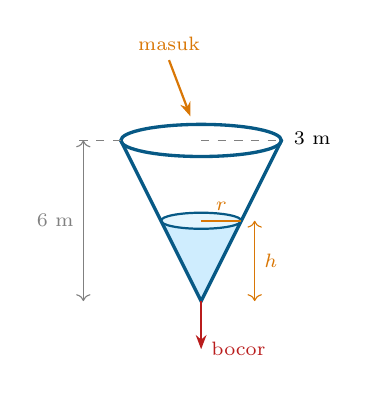
\begin{tikzpicture}[scale=0.68]
\fill[skyl!70] (-0.75,1.5)--(0,0)--(0.75,1.5) arc (0:-180:0.75 and 0.15)--cycle;
\draw[mainc,thick,fill=skyl!40] (0,1.5) ellipse (0.75 and 0.15);
\draw[mainc,very thick] (-1.5,3)--(0,0)--(1.5,3);
\draw[mainc,very thick] (0,3) ellipse (1.5 and 0.3);
\draw[ar,warmc] (-0.6,4.5)--(-0.2,3.45);
\node[font=\scriptsize,warmc,above] at (-0.6,4.5) {masuk};
\draw[ar,brick] (0,0)--(0,-0.9) node[right,font=\scriptsize,brick]{bocor};
\draw[<->,gray] (-2.2,0)--(-2.2,3) node[midway,left,font=\scriptsize]{$6$ m};
\draw[gray,dashed] (-1.5,3)--(-2.3,3);
\draw[gray,dashed] (0,3)--(1.5,3);
\node[font=\scriptsize,right] at (1.55,3.05) {$3$ m};
\draw[<->,warmc] (1.0,0)--(1.0,1.5) node[midway,right,font=\scriptsize,warmc]{$h$};
\draw[warmc,thick] (0,1.5)--(0.75,1.5) node[midway,above,font=\scriptsize,warmc]{$r$};
\end{tikzpicture}}}{\poin{8}}

\Needspace{26\baselineskip}
\tingkat{Tingkat HOTS}{soal 5}
\soal{\gbr{Gambar menunjukkan grafik $y=e^x$ dan sebuah garis lurus yang melalui titik asal $O$ dan menyinggung grafik di titik $T$.\par\smallskip
(a) Tentukan koordinat $T$ dan persamaan garis singgung tersebut.\par
(b) Buktikan bahwa $e^x\ge ex$ untuk setiap bilangan real $x$ dengan menganalisis $g(x)=e^x-ex$, dan tentukan kapan kesamaan terjadi.\par
(c) Dengan memilih $x=\dfrac\pi e$ pada (b), tentukan mana yang lebih besar, $e^{\pi}$ atau $\pi^{e}$.\par
(d) Untuk setiap bilangan real $k$, tentukan banyak solusi real persamaan $e^x=kx$. (Petunjuk: tulis $k=\dfrac{e^x}{x}$ dan selidiki grafik fungsi ini.)}{%
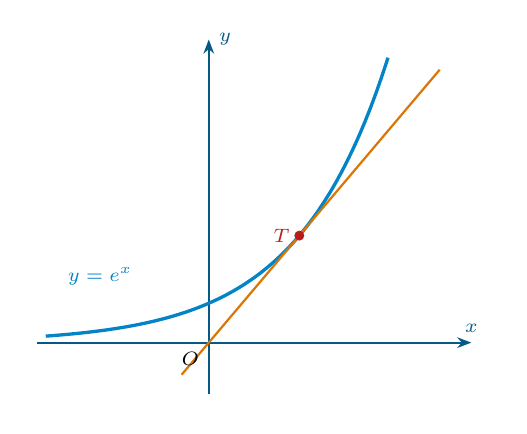
\begin{tikzpicture}[x=1.15cm,y=0.5cm]
\clip (-2.0,-1.6) rectangle (3.2,8.0);
\draw[ax] (-1.9,0)--(2.9,0) node[above,font=\scriptsize]{$x$};
\draw[ax] (0,-1.3)--(0,7.7) node[right,font=\scriptsize]{$y$};
\draw[accc,very thick,domain=-1.8:1.98,samples=60] plot(\x,{exp(\x)});
\draw[warmc,thick,domain=-0.3:2.55] plot(\x,{2.71828*\x});
\fill[brick] (1,2.71828) circle (1.8pt) node[left,font=\scriptsize]{$T$};
\node[font=\scriptsize,below left] at (0,0) {$O$};
\node[font=\scriptsize,accc,above] at (-1.2,1.2) {$y=e^x$};
\end{tikzpicture}}}{\poin{8}}

% =====================================================================
\newpage
\bagian{Kunci Jawaban dan Pembahasan Singkat}{Untuk guru dan pembahasan mandiri}
\par\vspace{0.6em}{\bfseries\color{mainc}Kunci Pilihan Ganda}\par\vspace{0.3em}
\small
\begin{tabularx}{\linewidth}{@{}*{10}{>{\centering\arraybackslash}X}@{}}\hline \textbf{1} & \textbf{2} & \textbf{3} & \textbf{4} & \textbf{5} & \textbf{6} & \textbf{7} & \textbf{8} & \textbf{9} & \textbf{10}\\ \hline E & C & A & B & {\scriptsize B,S,S,B} & D & B & A & D & C\\ \hline\end{tabularx}\\[6pt]
\begin{tabularx}{\linewidth}{@{}*{10}{>{\centering\arraybackslash}X}@{}}\hline \textbf{11} & \textbf{12} & \textbf{13} & \textbf{14} & \textbf{15} & \textbf{16} & \textbf{17} & \textbf{18} & \textbf{19} & \textbf{20}\\ \hline E & C & B & B & A & E & {\scriptsize B,S,B,S} & C & D & D\\ \hline\end{tabularx}
\par\vspace{0.4em}{\bfseries\color{mainc}Kunci Isian Singkat:}\ \ 1) $18$\quad 2) $32$\quad 3) $\sqrt{61}$\quad 4) $-\dfrac23$\quad 5) $2+2\ln2$
\par\vspace{0.8em}{\bfseries\color{mainc}\normalsize Pembahasan Pilihan Ganda}\par\vspace{0.2em}
\small\begin{enumerate}[leftmargin=2em,itemsep=2pt,topsep=2pt]
\item[\textbf{1.}] \textbf{(E)} Turunan di suatu titik sama dengan gradien garis singgung di titik itu. Garis $g$ melalui $(0,1)$ dan $(2,5)$, sehingga $f'(2)=\frac{5-1}{2-0}=2$. Karena $f(2)=5$, maka $f(2)+f'(2)=7$. (Jebakan: memakai angka $1$ sebagai gradien memberi $6$; memakai $\frac{\Delta x}{\Delta y}$ memberi $\frac{11}2$.)
\item[\textbf{2.}] \textbf{(C)} Sederhanakan dahulu: $x^3-8=(x-2)(x^2+2x+4)$, sehingga $f(x)=x^2+2x+4$ untuk $x\neq2$. Maka $f'(x)=2x+2$ dan $f'(1)=4$. (Aturan hasil bagi memberi hasil yang sama, tetapi lebih panjang.)
\item[\textbf{3.}] \textbf{(A)} $f'(x)=2\cos x+3\sin3x$. Di $x=\frac\pi2$: $2\cdot0+3\sin\frac{3\pi}2=3(-1)=-3$. (Jebakan: lupa faktor $3$ dari aturan rantai memberi $-1$; salah tanda memberi $3$.)
\item[\textbf{4.}] \textbf{(B)} Kecepatan $v(t)=s'(t)=3t^2-12t+9$, sehingga $v(2)=12-24+9=-3$. Tanda negatif berarti benda bergerak ke arah negatif dengan laju $3$ m/s. (Pengecoh: $s(2)=2$ adalah posisi, bukan kecepatan; $12$ muncul bila suku $+9$ terlupa.)
\item[\textbf{5.}] \textbf{(B, S, S, B)} Untuk $x\ge0$, $f(x)=x^2$; untuk $x<0$, $f(x)=-x^2$. (1) Kedua potongan menuju $0$ di $x=0$ dan $f(0)=0$, jadi $f$ kontinu: \textbf{B}. (2) $\frac{f(h)-f(0)}h=|h|\to0$ dari kiri maupun kanan, jadi turunan kiri $=$ turunan kanan $=0$: \textbf{S}. (3) Untuk $x<0$, $f'(x)=-2x$, sehingga $f'(-2)=4$, bukan $-4$: \textbf{S}. (4) $f'(x)=2x=2|x|$ untuk $x>0$, $f'(x)=-2x=2|x|$ untuk $x<0$, dan $f'(0)=0=2|0|$: \textbf{B}.
\item[\textbf{6.}] \textbf{(D)} $f'(x)=\dfrac{2\sin x\cos x}{2\sqrt{1+\sin^2x}}=\dfrac{\sin x\cos x}{\sqrt{1+\sin^2x}}$. Di $x=\frac\pi4$: $\dfrac{1/2}{\sqrt{3/2}}=\dfrac12\sqrt{\dfrac23}=\dfrac{\sqrt6}{6}$.
\item[\textbf{7.}] \textbf{(B)} Tanda $f'$: positif untuk $x<1$ (termasuk di kiri dan kanan $x=-2$, karena grafik hanya menyentuh sumbu $x$), negatif untuk $1<x<3$, positif untuk $x>3$. Jadi $f$ naik lalu turun di $x=1$ (maksimum lokal) dan turun lalu naik di $x=3$ (minimum lokal). Di $x=-2$ nilai $f'=0$ tetapi tanda tidak berubah, sehingga bukan titik ekstrem.
\item[\textbf{8.}] \textbf{(A)} Turunkan implisit: $3y^2y'+y+xy'=4x$, sehingga $y'=\dfrac{4x-y}{3y^2+x}$. Di $(1,1)$: $y'=\frac34$. Gradien normal $=-\frac43$: $y-1=-\frac43(x-1)\Rightarrow 4x+3y=7$. (Pilihan B adalah persamaan garis singgungnya.)
\item[\textbf{9.}] \textbf{(D)} $P'(x)=2x\,f(g(x))+x^2\,f'(g(x))\,g'(x)$. Di $x=2$: $g(2)=1$, sehingga $f(g(2))=f(1)=2$ dan $f'(g(2))=f'(1)=4$; $g'(2)=6$. $P'(2)=4\cdot2+4\cdot4\cdot6=8+96=104$. (Jebakan: memakai $f'(2)=-2$ memberi $-40$; melupakan $g'$ memberi $24$.)
\item[\textbf{10.}] \textbf{(C)} $f'(x)=3x^2+2ax+3a\ge0$ untuk semua $x$ bila diskriminan $\le0$: $4a^2-36a\le0\Rightarrow0\le a\le9$. Nilai $a=0$ dan $a=9$ tetap dihitung karena $f'=0$ hanya di satu titik (masing-masing $f'=3x^2$ dan $f'=3(x+3)^2$), sehingga $f$ tetap monoton naik. Banyaknya: $10$.
\item[\textbf{11.}] \textbf{(E)} $f'(x)=\dfrac{2e^{2x}-2e^{-2x}}{e^{2x}+e^{-2x}}$. Di $x=\ln\sqrt3$: $e^{2x}=3$ dan $e^{-2x}=\frac13$, sehingga $f'=\dfrac{6-\frac23}{3+\frac13}=\dfrac{16/3}{10/3}=\dfrac85$. (Jebakan: lupa faktor $2$ dari aturan rantai memberi $\frac45$.)
\item[\textbf{12.}] \textbf{(C)} Titik belok: $f''(1)=0\Rightarrow6a+2b=0\Rightarrow b=-3a$. $f'(1)=-3\Rightarrow3a+2b+c=-3\Rightarrow c=3a-3$. $f(0)=5\Rightarrow d=5$. $f(1)=3\Rightarrow a+b+c+d=a+2=3\Rightarrow a=1$. Jadi $f(x)=x^3-3x^2+5$. $f'(x)=3x(x-2)$: stasioner di $x=0$ ($f''=-6<0$, maksimum lokal $f(0)=5$) dan $x=2$ ($f''=6>0$, minimum lokal $f(2)=1$). Selisih $5-1=4$.
\item[\textbf{13.}] \textbf{(B)} Garis singgung $y=x^2$ di $x=p$ adalah $y=2px-p^2$. Garis ini menyinggung parabola kedua bila $-(x-2)^2=2px-p^2$ mempunyai tepat satu akar, yaitu $x^2+(2p-4)x+4-p^2=0$ berdiskriminan nol: $(2p-4)^2-4(4-p^2)=8p^2-16p=0\Rightarrow p=0$ atau $p=2$. Diperoleh $\ell_1:y=0$ dan $\ell_2:y=4x-4$. Titik sudut segitiga: $(0,0)$, $(0,-4)$, dan $(1,0)$ (perpotongan $\ell_1$ dan $\ell_2$). Luas $=\frac12\cdot4\cdot1=2$.
\item[\textbf{14.}] \textbf{(B)} Misalkan $x$ jarak Dina dari tiang dan $s$ panjang bayangan. Segitiga sebangun: $\dfrac{s}{1{,}5}=\dfrac{x+s}{6}\Rightarrow4{,}5s=1{,}5x\Rightarrow s=\dfrac x3$. Maka $\dd st=\dfrac13\dd xt=\dfrac13(1{,}2)=0{,}4$ m/s. Lajunya tetap, sehingga data ``$9$ m'' tidak diperlukan. (Pengecoh: $1{,}6$ m/s adalah laju \emph{ujung} bayangan, $\frac43\cdot1{,}2$.)
\item[\textbf{15.}] \textbf{(A)} Tinggi trapesium $10\sin\theta$, sisi atas $10+20\cos\theta$. Luas $A(\theta)=\frac12(20+20\cos\theta)(10\sin\theta)=100\sin\theta(1+\cos\theta)$. $A'(\theta)=100(\cos\theta+\cos^2\theta-\sin^2\theta)=100(2\cos^2\theta+\cos\theta-1)=100(2\cos\theta-1)(\cos\theta+1)$. Pada $0<\theta<\frac\pi2$, $A'=0$ hanya saat $\cos\theta=\frac12$, yaitu $\theta=\frac\pi3$, dan di situ $A'$ berubah dari $+$ ke $-$. $A\!\left(\frac\pi3\right)=100\cdot\frac{\sqrt3}2\cdot\frac32=75\sqrt3$. (Pengecoh: $\theta=\frac\pi2$ memberi penampang persegi dengan luas $100$ yang lebih kecil.)
\item[\textbf{16.}] \textbf{(E)} $f(0)=b=-2$. $f'(x)=(a-b-ax)e^{-x}$, dan $f'(3)=0\Rightarrow-2a-b=0\Rightarrow a=1$. Jadi $f(x)=(x-2)e^{-x}$. $f'(x)=(3-x)e^{-x}$ dan $f''(x)=(x-4)e^{-x}$, yang berubah tanda di $x=4$. Ordinat titik belok $f(4)=2e^{-4}=\dfrac2{e^4}$.
\item[\textbf{17.}] \textbf{(B, S, B, S)} (1) $P$ adalah minimum lokal dan kurva cekung ke atas di sana: $f'=0$, $f''>0$, \textbf{B}. (2) Antara minimum $P$ dan maksimum $R$ kurva naik, jadi di $Q$ berlaku $f'>0$ (bukan negatif), \textbf{S}. (3) $R$ maksimum lokal: $f'=0$, $f''<0$, \textbf{B}. (4) Di $S$ kurva naik ($f'>0$) dan cekung ke atas ($f''>0$), sehingga $f''<0$ salah, \textbf{S}. (Grafik yang dipakai: $f(x)=\frac{x^4}4-\frac{x^2}2$.)
\item[\textbf{18.}] \textbf{(C)} $f'(x)=2\sin x\cos x=\sin2x$, $f''=2\cos2x$, $f'''=-4\sin2x$, dan seterusnya. Pola umum: $f^{(n)}(x)=2^{n-1}\sin\!\big(2x+\tfrac{(n-1)\pi}2\big)$. Untuk $n=2025$ dan $x=\frac\pi4$: sudutnya $\frac\pi2+1012\pi$, sehingga $\sin=1$ dan nilainya $2^{2024}$. (Cek: nilai $f^{(n)}(\frac\pi4)$ untuk $n=1,3,5,7$ adalah $1,-4,16,-64$, yaitu $(-4)^{(n-1)/2}$; untuk $n=2025$ hasilnya $(-4)^{1012}=2^{2024}$.)
\item[\textbf{19.}] \textbf{(D)} Grafik kubik ($a\neq0$) punya tepat satu titik belok di $x=-\frac b{3a}$, karena $f''(x)=6ax+2b$ berubah tanda di sana; bila $a=0$ grafik berupa parabola, garis, atau konstanta, yang tidak mempunyai titik belok. Jadi pertanyaan ekuivalen dengan ``apakah $a\neq0$?''. Pernyataan (1): bila $a=0$ maka $f'(x)=2bx+c$ hanya punya paling banyak satu akar (atau tak hingga), tidak mungkin tepat dua; jadi $a\neq0$, cukup. Pernyataan (2): fungsi berderajat $\le2$ tidak mungkin punya tepat tiga akar berbeda; jadi $a\neq0$, cukup. Masing-masing cukup.
\item[\textbf{20.}] \textbf{(D)} Biaya $C(x)=3x+5\sqrt{36+(8-x)^2}$ (juta rupiah) dengan $x=AP$, $0\le x\le8$. $C'(x)=3-\dfrac{5(8-x)}{\sqrt{36+(8-x)^2}}=0\Rightarrow5(8-x)=3\sqrt{36+(8-x)^2}$. Kuadratkan dengan $u=8-x$: $25u^2=9(36+u^2)\Rightarrow16u^2=324\Rightarrow u=\frac92$, sehingga $x=3{,}5$ km. Maka panjang kabel laut $\sqrt{36+4{,}5^2}=7{,}5$ km dan $C(3{,}5)=3(3{,}5)+5(7{,}5)=48$. Pembanding di ujung: $C(0)=50$ (langsung dari $A$ ke $B$ lewat laut) dan $C(8)=54$ (seluruhnya menyusuri pantai). Minimum $=48$ juta rupiah.
\end{enumerate}
\par\Needspace{6\baselineskip}\vspace{0.6em}{\bfseries\color{mainc}\normalsize Pembahasan Isian Singkat}\par\vspace{0.2em}
\small\begin{enumerate}[leftmargin=2em,itemsep=2pt,topsep=2pt]
\item[\textbf{1.}] \textbf{Jawaban: $18$.} $v(t)=6t^2-42t+60=6(t-2)(t-5)$, sehingga partikel berhenti sesaat di $t=2$ dan $t=5$. Percepatan $a(t)=12t-42$, dan pada kali kedua ($t=5$): $a=60-42=18$ m/s$^2$.
\item[\textbf{2.}] \textbf{Jawaban: $32$.} Gradien garis $=9$, sehingga $3x^2-6x=9\Rightarrow x^2-2x-3=0\Rightarrow x=3$ atau $x=-1$. Di $(3,0)$: $0=27+k\Rightarrow k=-27$. Di $(-1,-4)$: $-4=-9+k\Rightarrow k=5$. Selisih $5-(-27)=32$.
\item[\textbf{3.}] \textbf{Jawaban: $\sqrt{61}$.} Tulis $f(x)=\sqrt{(x-0)^2+(0-2)^2}+\sqrt{(x-6)^2+(0-3)^2}$, yaitu jumlah jarak titik $(x,0)$ ke $(0,2)$ dan ke $(6,3)$. Dengan turunan: $f'(x)=\dfrac{x}{\sqrt{x^2+4}}-\dfrac{6-x}{\sqrt{(6-x)^2+9}}=0\Rightarrow\dfrac x2=\dfrac{6-x}3\Rightarrow x=\dfrac{12}5$ (kuadratkan lalu ambil akar positif). Nilai minimum: $f\!\left(\frac{12}5\right)=\sqrt{\frac{244}{25}}+\sqrt{\frac{549}{25}}=\frac{2\sqrt{61}}5+\frac{3\sqrt{61}}5=\sqrt{61}$. (Cara lain: cerminkan $(0,2)$ menjadi $(0,-2)$; jarak ke $(6,3)$ adalah $\sqrt{6^2+5^2}=\sqrt{61}$.)
\item[\textbf{4.}] \textbf{Jawaban: $-\frac23$.} Turunkan implisit: $2x-y-xy'+2yy'=0\Rightarrow y'=\dfrac{y-2x}{2y-x}$. Di $P(1,2)$: $y'=\dfrac{2-2}{4-1}=0$ (garis singgung mendatar). Turunkan sekali lagi: $y''=\dfrac{(y'-2)(2y-x)-(y-2x)(2y'-1)}{(2y-x)^2}$. Di $P$: $y''=\dfrac{(0-2)(3)-0}{9}=-\dfrac23$. Karena $y'=0$ dan $y''<0$, $P$ adalah titik tertinggi kurva (sesuai gambar).
\item[\textbf{5.}] \textbf{Jawaban: $2+2\ln2$.} Turunan logaritmik: $\ln f=x\ln(x^2+1)\Rightarrow\dfrac{f'}f=\ln(x^2+1)+\dfrac{2x^2}{x^2+1}$. Di $x=1$: $f(1)=2$ dan $\dfrac{f'(1)}{2}=\ln2+1$, sehingga $f'(1)=2\ln2+2$.
\end{enumerate}
\par\Needspace{8\baselineskip}\vspace{0.6em}{\bfseries\color{mainc}\normalsize Pembahasan dan Pedoman Penskoran Uraian}\par\vspace{0.2em}
\small\begin{enumerate}[leftmargin=2em,itemsep=3pt,topsep=2pt]
\item[\textbf{1.}] (a) Keliling kerangka: $2r+2h+\pi r=10\Rightarrow h=\dfrac{10-(2+\pi)r}{2}$. Luas $A=2rh+\dfrac12\pi r^2=r\big(10-(2+\pi)r\big)+\dfrac{\pi r^2}2=10r-\dfrac{4+\pi}2r^2$. Batas: $h\ge0\Rightarrow0<r\le\dfrac{10}{2+\pi}$. (b) $A'(r)=10-(4+\pi)r=0\Rightarrow r=\dfrac{10}{4+\pi}$ ($\approx1{,}4$ m, memenuhi batas). $A''(r)=-(4+\pi)<0$, jadi $A$ maksimum. (c) $A_{\max}=10r-\dfrac{4+\pi}2r^2=\dfrac{100}{4+\pi}-\dfrac{50}{4+\pi}=\dfrac{50}{4+\pi}\approx7{,}0$ m$^2$. Tinggi: $h=\dfrac{10-(2+\pi)r}2=\dfrac{10\big(4+\pi-2-\pi\big)}{2(4+\pi)}=\dfrac{10}{4+\pi}=r$. (d) Di $r\to0$: $A\to0$. Di $r=\frac{10}{2+\pi}$ ($h=0$, jendela hanya setengah lingkaran): $A=\dfrac{\pi r^2}2=\dfrac{50\pi}{(2+\pi)^2}\approx5{,}9$. Keduanya lebih kecil dari $7{,}0$, sehingga maksimum di (b) adalah maksimum mutlak. \\ \textit{Penskoran: tiap bagian 2 poin.}
\item[\textbf{2.}] (a) $T'(t)=75\cdot\left(-\dfrac1{10}\right)e^{-t/10}=-7{,}5e^{-t/10}$. $T'(0)=-7{,}5$ berarti pada saat awal suhu teh turun dengan laju sesaat $7{,}5^\circ$C per menit. (b) Laju penurunan $3{,}75$ berarti $T'(t)=-3{,}75\Rightarrow e^{-t/10}=\frac12\Rightarrow t=10\ln2\approx6{,}9$ menit. Suhu saat itu: $25+75\cdot\frac12=62{,}5^\circ$C. (c) $T''(t)=0{,}75e^{-t/10}>0$ untuk semua $t$. Artinya $T'$ naik menuju $0$ dari bawah: laju penurunan suhu makin kecil, sehingga pendinginan makin lambat; grafik cekung ke atas. (d) Garis singgung di $t=0$: $T=100-7{,}5t$. Untuk $T=25$: $t=10$. Karena grafik cekung ke atas, kurva selalu berada di atas garis singgungnya, sehingga $T(10)=25+75e^{-1}\approx52{,}6>25$; teh masih jauh lebih panas dari ruangan. \\ \textit{Penskoran: tiap bagian 2 poin.}
\item[\textbf{3.}] (a) $y'=-\dfrac1{x^2}$, sehingga gradien di $P$ adalah $-\dfrac1{t^2}$. Persamaan: $y-\dfrac1t=-\dfrac1{t^2}(x-t)\Rightarrow y=-\dfrac x{t^2}+\dfrac2t$. (b) $y=0$: $x=2t$, jadi $A(2t,0)$. $x=0$: $y=\dfrac2t$, jadi $B\!\left(0,\dfrac2t\right)$. Titik tengah $AB$: $\left(t,\dfrac1t\right)=P$. (c) Luas $\triangle OAB=\dfrac12\cdot2t\cdot\dfrac2t=2$, tidak bergantung pada $t$. (d) $AB^2=(2t)^2+\left(\dfrac2t\right)^2=4t^2+\dfrac4{t^2}$. Turunan: $8t-\dfrac8{t^3}=0\Rightarrow t^4=1\Rightarrow t=1$ (karena $t>0$). Tanda turunan berubah dari $-$ ke $+$ di $t=1$, jadi minimum. $AB^2=8\Rightarrow AB_{\min}=2\sqrt2$. \\ \textit{Penskoran: tiap bagian 2 poin.}
\item[\textbf{4.}] (a) Perbandingan segitiga sebangun: $\dfrac rh=\dfrac36\Rightarrow r=\dfrac h2$. $V=\dfrac13\pi r^2h=\dfrac13\pi\cdot\dfrac{h^2}4\cdot h=\dfrac\pi{12}h^3$. (b) Laju bersih: $\dd Vt=2-\dfrac h2$. Aturan rantai: $\dd Vt=\dfrac\pi4h^2\dd ht$. Jadi $\dd ht=\dfrac{2-\frac h2}{\frac\pi4h^2}=\dfrac{8-2h}{\pi h^2}$. Untuk $h=2$: $\dd ht=\dfrac{4}{4\pi}=\dfrac1\pi$ m/menit. (c) Luas permukaan $L=\pi r^2=\dfrac{\pi h^2}4$, sehingga $\dd Lt=\dfrac{\pi h}2\dd ht$. Untuk $h=2$: $\dd Lt=\pi\cdot\dfrac1\pi=1$ m$^2$/menit. (d) $\dd ht=0\Rightarrow8-2h=0\Rightarrow h=4$ m. Untuk $h<4$, $\dd ht>0$ (air naik, makin lambat), dan di $h=4$ laju masuk sama dengan laju bocor, sehingga tinggi air menuju $4$ m dan tidak melampauinya. Karena $4<6$, tangki \textbf{tidak meluap}. \\ \textit{Penskoran: (a) 1 poin; (b) 3 poin; (c) 2 poin; (d) 2 poin.}
\item[\textbf{5.}] (a) Garis singgung di $x=a$: $y=e^a(x-a)+e^a$. Melalui $O$: $0=e^a(1-a)\Rightarrow a=1$. Jadi $T(1,e)$ dan garisnya $y=ex$. (b) $g(x)=e^x-ex$, $g'(x)=e^x-e$. $g'<0$ untuk $x<1$ dan $g'>0$ untuk $x>1$, jadi $g$ mempunyai minimum mutlak di $x=1$ dengan $g(1)=0$. Maka $g(x)\ge0$, yaitu $e^x\ge ex$, dengan kesamaan hanya di $x=1$. (c) Ambil $x=\frac\pi e\ne1$: $e^{\pi/e}>e\cdot\frac\pi e=\pi$. Pangkatkan keduanya dengan $e>0$: $e^\pi>\pi^e$. Jadi $e^\pi$ lebih besar. (d) $x=0$ bukan solusi sehingga $k=\varphi(x)=\dfrac{e^x}x$, dengan $\varphi'(x)=\dfrac{e^x(x-1)}{x^2}$. Untuk $x>0$: $\varphi$ turun pada $(0,1)$ dan naik pada $(1,\infty)$, bernilai minimum $\varphi(1)=e$, dan $\varphi\to\infty$ saat $x\to0^+$ maupun $x\to\infty$. Untuk $x<0$: $\varphi<0$ dan $\varphi'<0$, turun dari $0^-$ (saat $x\to-\infty$) ke $-\infty$ (saat $x\to0^-$), sehingga memuat setiap nilai negatif tepat sekali. Kesimpulan: $k<0$: $1$ solusi; $0\le k<e$: tidak ada solusi; $k=e$: $1$ solusi; $k>e$: $2$ solusi. \\ \textit{Penskoran: tiap bagian 2 poin.}
\end{enumerate}
\end{document}
